\documentclass[a4paper,12pt]{book}

%Pacchetti utili
%************
%* packages *
%************

%Codifica
\usepackage[utf8]{inputenc}

%Lingua, sostituire italian con english nel caso in cui la tesi sia scritta in inglese
\usepackage[english]{babel}

%Pacchetto per definire layout di pagina
\usepackage{fancyhdr}
\usepackage{sectsty}
\usepackage[left=3cm, right=3cm, bottom=3cm]{geometry}

%Spazia linee all'interno del documento
\usepackage{setspace}

%Listati di codice
\usepackage{verbatim}
\usepackage{listings}

%Didascalie immagini
\usepackage[hang,small,sf,font=scriptsize, labelfont=bf]{caption}
\usepackage{subcaption}

%Inclusione immagini
\usepackage{graphicx}
\graphicspath{{images/}}

%Impostazioni note a piè pagina
\usepackage[stable]{footmisc}

%Citazioni e riferimenti a label
\usepackage{cite}
\usepackage[english]{varioref}

%Colori
\usepackage[usenames]{color}
\usepackage{xcolor}
\usepackage{colortbl}

%Crea link ipertestuali
\usepackage[hidelinks]{hyperref}

%Formattazione url
\usepackage{url}

%Inserimento formule
% \usepackage{amsmath}
% \usepackage{mathrsfs}

%Inserimento pseudocodice
% \usepackage{algorithm}
% \usepackage{algpseudocode}

%Citazione frasi
% \usepackage{csquotes}

%Inserimento di Lorem ipsum nel testo
% \usepackage{lipsum}

%\usepackage{lmodern}

\usepackage{enumitem}

% to render pdf/a
\usepackage[a-1b]{pdfx}


%Nuovi comandi
% %*****************
%* nuovi comandi *
%*****************

\newcommand{\abs}[1]{\left|#1\right|}                               % modulo
\newcommand{\dato}{\left|\right.}                                   % probabilit\`{a} condizionata
\newcommand{\fun}[1]{\mathrm{#1}}                                   % stile funzione
\newcommand{\imp}{\;\;\Longrightarrow\;\;}                          % implicazione
\newcommand{\norma}[1]{\left\| #1 \right\|}                         % norma
\newcommand{\prob}[1]{\mathrm{P}\!\left[#1\right]}                  % probabilit\`{a}
\newcommand{\expect}[1]{\mathrm{E}\!\left[#1\right]}                % aspettazione
\newcommand{\sse}{\;\;\Longleftrightarrow\;\;}                      % se e solo se
\newcommand{\vect}[1]{{\boldsymbol{\mathrm{#1}}}}                   % stile vettore
\newcommand{\real}[1]{\fun{Re}\left[#1\right]}                      % parte reale
\newcommand{\imag}[1]{\fun{Im}\left[#1\right]}                      % parte immaginaria
\newcommand{\Dim}[1]{\fun{dim}\left[#1\right]}                      % dimensione di una matrice
\newcommand{\Det}[1]{\fun{det}\left[#1\right]}                      % determinante di una matrice
\newcommand{\Ker}[1]{\fun{ker}\left[#1\right]}                      % ker di una matrice
\newcommand{\rango}[1]{\fun{rango}\left[#1\right]}                  % rango di una matrice
\newcommand{\scalare}[2]{\left\langle #1, #2 \right\rangle}         % prodotto scalare
\newcommand{\blbrace}{\left  \lbrace}                               % parentesi graffa sinistra grande
\newcommand{\brbrace}{\right \rbrace}                               % parentesi graffa destra grande
\newcommand{\sinc}{\fun{sinc}}                                      % sinc
\newcommand{\rect}{\fun{rect}}                                      % rect
\newcommand{\rcos}{\fun{rcos}}                                      % rcos
\newcommand{\sgn}{\fun{sgn}}                                        % sgn
\newcommand{\N}{\mathbb{N}}                                         % insieme dei numeri naturali
\newcommand{\Z}{\mathbb{Z}}                                         % insieme dei numeri interi
\newcommand{\Q}{\mathbb{Q}}                                         % insieme dei numeri razionali
\newcommand{\R}{\mathbb{R}}                                         % insieme dei numeri reali
\newcommand{\C}{\mathbb{C}}                                         % insieme dei numeri complessi
\newcommand{\seq}[2][n]{#2_{0}, #2_{1}, \ldots, \, #2_{#1}}         % sequenza
\newcommand{\Span}[2][n]
{\fun{span} \blbrace #2_{1}, #2_{2}, \ldots, \, #2_{#1} \brbrace}   % spazio generato
\newcommand{\ddt}{\frac{\fun{d}}{\fun{dt}}}                         % derivata
\newcommand{\Div}[2]{#1 \; \mid \; #2}                              % divide
\newcommand{\MCD}[2]{\fun{MCD}\(#1, #2\)}                           % massimo comun divisore
\newcommand{\mcm}[2]{\fun{mcm}\(#1, #2\)}                           % minimo comune multiplo
\newcommand{\goodgap}{
                      \hspace{\subfigtopskip}
                      \hspace{\subfigbottomskip}
                     }                                              % interlinea opportuna per le sottofigure
\newcommand{\eng}[1]{\emph{#1}}                                   % inglese
\newcommand{\virg}[1]{``#1"}                                        % fa una citazione tra virgolette
%\newcommand{\unit}[2]($\frac{\text{#1}}{\text{#2}}$)                % unit\`{a} di misura
\newcommand{\textttvar}[1]{{\ttvar #1}}

\definecolor{gray}{gray}{0.9}
\newcommand{\listato}[1]{\lstset{language=#1, numbers=left, numberstyle=\tiny, stepnumber=2, numbersep=5pt, numberblanklines=false, xleftmargin=5pt, captionpos=b, stringstyle=\ttfamily, columns=flexible, showstringspaces=false, tabsize=2, frame=single, framerule=0pt, backgroundcolor=\color{gray}, basicstyle=\small}}

%****************************
%* ridefinizioni di comandi *
%****************************

\renewcommand{\(}{\left(}                                     % parentesi tonda sinistra grande
\renewcommand{\)}{\right)}                                    % parentesi tonda destra grande
\renewcommand{\[}{\left[}                                     % parentesi quadra sinistra grande
\renewcommand{\]}{\right]}                                    % parentesi quadra destra grande
\renewcommand{\exp}[1]{\fun{e}^{#1}}                          % esponenziale
\renewcommand{\gcd}[2]{\fun{gcd}\(#1, #2\)}                   % massimo comun divisore

\renewcommand{\lstlistingname}{Listing}
\renewcommand{\lstlistlistingname}{Elenco dei listati codice}

\makeatletter
\def\BState{\State\hskip-\ALG@thistlm}
\makeatother

%Definizione input e output pseudocodice
\renewcommand{\algorithmicrequire}{\textbf{Input:}}
\renewcommand{\algorithmicensure}{\textbf{Output:}}
 
%"Nome" della bibliografia
\addto{\captionsenglish}{%
  \renewcommand{\bibname}{References}
}

%Impostazioni dei margini, definizione di colori e di stili vari
\newfont{\ttvar}{cmvtt10 scaled 1200}     % nuovo carattere tipi courier a spaziatura variabile per le dimostrazioni

% margini senato
\textwidth       =  14.50 cm            % larghezza 21 cm - 4 cm (sinistro) - 2.5 (destro)
\textheight      =  23.10 cm            % altezza 29.7 cm - 3 cm (superiore) - 2 (inferiore)
\topmargin       =   0.00 cm            % margine superiore 3 cm diminuito di 1 inch
\oddsidemargin   =   1.46 cm            % margine sinistro 4 cm diminuito di 1 inch
\evensidemargin  =  -0.04 cm            % margine destro 2.5 cm diminuito di un inch

\setlength{\headsep}{1.0cm}
\setlength{\footskip}{1.0cm}
\parindent = 0.7cm
\captionmargin = 0.7cm

%Interlinea 1.5
\onehalfspacing

% stile pagina
\pagestyle{fancy}
\renewcommand{\chaptermark}[1]{\markboth{\chaptername\ \thechapter.\ #1 }{}}
\renewcommand{\sectionmark}[1]{\markright{\thesection\ #1}{}}
\fancyhead{}
\fancyhead[LE,RO]{\sffamily \thepage}
\fancyhead[RE]{\sffamily \leftmark}
\fancyhead[LO]{\sffamily \rightmark}
\fancyfoot{}

% ridefinisco lo stile plain
\fancypagestyle{plain}{ \fancyhead{} \fancyfoot{}
\fancyfoot[C]{\sffamily \thepage}
\renewcommand{\headrulewidth}{0pt}}

% stile per i titoli
\allsectionsfont{\sffamily \raggedright}

% definisco i colori
\definecolor{codegreen}{rgb}{0,0.6,0}
\definecolor{codegray}{rgb}{0.5,0.5,0.5}
\definecolor{codepurple}{rgb}{0.58,0,0.82}
\definecolor{backcolour}{rgb}{0.95,0.95,0.92}
\definecolor{backcolourwhite}{rgb}{1,1,1}

%definisco stile listati di codice
\lstdefinestyle{mystyle}{
    backgroundcolor=\color{backcolour},   
    commentstyle=\color{codegreen},
    keywordstyle=\color{magenta},
    numberstyle=\tiny\color{codegray},
    stringstyle=\color{codepurple},
    basicstyle=\ttfamily\footnotesize,
    breakatwhitespace=false,         
    breaklines=true,                 
    captionpos=b,                    
    keepspaces=true,                 
    numbers=left,                    
    numbersep=5pt,                  
    showspaces=false,                
    showstringspaces=false,
    showtabs=false,                  
    tabsize=2
}

\lstset{style=mystyle}
\lstset{emph={RandomForestClassifier, RandomizedSearchCV, GridSearchCV},emphstyle=\underbar}



\begin{document}

\begin{titlepage}
\begin{center}

\includegraphics[scale=0.1]{images/logo.png}\\

%Per il frontespizio del dipartimenti di Ing. dell'Informazione commentare le riga precedente e decommentare la successiva
%\includegraphics[scale=0.2]{images/logo_unipd.png} \hfill \includegraphics[scale=0.2]{images/logo_dei.png}\\
\vspace{0.8cm}
\textsc{\LARGE Universit\`{a} degli Studi di Padova}\\
\vspace{0.45cm}
\textsc{\large Dipartimento di Ingegneria dell'Informazione}\\
\vspace{0.4cm}
\textsc{\large Corso di Laurea Triennale in}\\
\textsc{\large Ingegneria Informatica}\\
\vfill
% Title
{ \LARGE \bfseries The Importance of a Plaform-Agnosting Bytecode for a Decentralized Network
}\\
\vfill
\textit{\large Relatore:} \hfill \textit{\large Laureando:}\\
\textsc{\large Prof. Luca Boldrin} \hfill \textsc{Gabriele Miotti}\\
\hfill \textsc{2000165}\\

\vfill
% Bottom of the page
{\large Anno Accademico 2022/2023}
\end{center}
\end{titlepage}

\thispagestyle{empty} %pagina bianca dopo il titolo
\cleardoublepage

\pagenumbering{roman} %numerazione romana per l'indice, l'abstract e i ringraziamenti
\thispagestyle{empty}

\clearpage{\pagestyle{plain}\cleardoublepage}
%definisco il layout dell'abstract
\def\changemargin#1#2{\list{}{\rightmargin#2\leftmargin#1}\item[]}
\let\endchangemargin=\endlist 

%Genero l'ambiente per l'abstract
\newcommand\summaryname{Abstract}
\newenvironment{Abstract}%
    {\begin{center}%
    \bfseries{\summaryname} \end{center}}
    
\begin{Abstract}
How can a distributed network agree on the execution of an arbitrary code in a trust-free way? Currently there are plenty of solutions to achieve that. Every solution differs by the network's structure and protocols but the common ground is the presence of a bytecode that is able to run arbitrary code in a deterministic manner. This paper will describe the basic characteristics of a Platform Agnostic Bytecode and how is used in Polkadot, a distributed network that `aims to provide a scalable and interoperable framework for multiple chains with pooled security`~\cite{burdges2020overview}.
\end{Abstract}


\clearpage{\pagestyle{plain}\cleardoublepage}
\tableofcontents %Indice

\clearpage{\pagestyle{plain}\cleardoublepage} %Numerazione araba per i capitoli
\pagenumbering{arabic}

\clearpage{\pagestyle{plain}\cleardoublepage} %Comando per iniziare il capitolo su pagina dispari
\chapter{PAB} %Nome capitolo
\label{chapter:pab} %Label per creare riferimenti al capitolo
\documentclass[../main.tex]{subfiles}
\graphicspath{{\subfix{../images/}}}

\begin{document}

\section{Platform-Agnostic Bytecode}
\subsection{Definition}

A Platform-Agnostic Bytecode (PAB) is a bytecode that follows those two main principles:

\begin{itemize}
    \item Turing Completness
    \item Support for tooling that makes it exacutable on every machine
\end{itemize}

A bytecode like this ideally is designed to be executed on a virtual machine that follows general patters. This design should make easier the compilation to another real machine's bytecode. Examples of real architectures with specified bytecode are AMD and Intel with x86 or ARM with aarch64. % TODO: check this last sentence

\subsection{Execution}

PABs require multiple phases of Compilation, the first one is encountered when you want to compile your High-Level language to the PAB using a Cross-Compiler. Once you have the arbitrary PAB code, you should be able to run it on every machine using another compiler that will create the final executable code.

Re-compiling is not the only way to execute a PAB, another common solution is to implement a VirtualMachine (VM) able to run aribitrary PAB code interpreting it.

\subsection{Key features}

Every bytecode can be a PAB if tools to make it runnable to different machine exist. Every bytecode, ideally, can become a PAB then there must be some metrics to define which one is the better PAB, those are:

\begin{description}[style=nextline]
  \item[Hardware Independence]
        A bytecode can't be a PAB if tightly related to specific hardware. A PAB can be defined as such if there is no direct connection between bytecode and hardware, the only exception is if there is a small relationship but the execution on different hardware requires only little overhead.
  \item[Sandboxing]
        The machine used to execute the PAB is defined as \textit{embedder}. The embedder will execute arbitrary code, possibly malicious, and avoiding any security problem is the aim of the embedder, sandobxing is the solution.
        Executing the PAB in a sandboxed environment makes impossible to compromise the embedder, the implementation of the sandboxed environment is embedder dependent but a PAB can be more or less suitable for this feature.
  \item[Efficency]
        The efficency of a PAB has a lot of meaning, it could be:

        \begin{itemize}
          \item Compiling High-Level Language to the PAB
          \item Execution of the PAB, it could mean compile to the final bytecode and then execute it, interpret it or more complex solution
        \end{itemize}

        Generally the first is not really related to the PAB, but more on the tools used (examples gcc, rustc, etc.). The execution efficiency is the real deal, how fast a PAB can be executed on a machine is crucial.
  \item[Tool Simlicity]
        The easyness of compiling an High-Level language and the executing the PAB is very important to make a it usable in the real world.
  \item[Support as Compilation Target]
        Writing bytecode by hand (or any text representation) is something really rare and done only in specific cases. Every compiled language has a compiler to make this, and is very important for a PAB to support the compilation from as many languages as possible.
  % TODO: there are others important factors?
\end{description}

\subsection{Current usage}

PAB are widely used and the following are a couple of examples:

\begin{description}[style=nextline]
  \item[JVM]
  LOL
  \item[eBPF]
  Linux brought eBPF into the kernel, enabling arbitrary programs to be executed in a privileged context (OS level).
  \item[LLVM IR]
  LLVM IR is the LLVM assembly language, it provides type safety, low-level operations, flexibility, and the capability of representing ‘all’ high-level languages cleanly. It is the common code representation used throughout all phases of the LLVM compilation strategy. \href{https://llvm.org/docs/LangRef.html\#abstract)}{llvm}
  \item[WASM]
  WebAssembly is a safe, portable, low-level code format designed for efficient execution and compact representation \href{https://webassembly.github.io/spec/core/}{wasm-spec}
\end{description}

\subsection{PAB in blockchains}

Blockchains are Distributes Systems that needs to agree on the execution of arbitrary code (more or less, TODO: explain better) and the code has to run on different machines. PAB is the solution for both problem, but there is a little caveat in the first problem: the code execution must arrive at the same result, regardless of the machine the code is running on. What has just been described will be called \"execution determinism\" from now on.

\end{document}


\clearpage{\pagestyle{plain}\cleardoublepage}
\chapter{Wasm}
\label{chapter:wasm}
\documentclass[../main.tex]{subfiles}

\begin{document}

\section{WASM}
\subsection{Definitions}

WebAssembly, shortened to Wasm, is a binary instruction format for a stack-based virtual machine ~\cite{wasm-core-spec}. It is a platform-agnostic binary format, meaning that it will run the same exact instructions across whatever machine it operates on. ~\cite{wasm-polkadot-wiki}

`asm.js` was Wasm precursor, but browser vendors like Mozilla, Google, Microsoft, and Apple focused on the Wasm design. The main goal was to create a binary format with some mandatory features: compact, support for streaming compilation and sanboxed execution.

Wasm is currently a compilation target for a lot of high level language. This allows many different languages to enter the web-world, in both client and server sides, but also in completely different applications.

Examples are plugins, imagine an application able to execute custom script developed by the user, if those scripts are in Wasm then the High-Level language used to develop those plugins is not constrained to a single one but to all the languages that are able to compile to Wasm.

Wasm main design goals, as specified in the Wasm specification introduction ~\cite{wasm-core-spec}, are:
\begin{description}[font=$\bullet$ \scshape\bfseries]
  \item[Fast] Its design allows to create executors with so less overhead that the execution is almost as fast as native code
  \item[Safe] It is completely memory-safe as long as the executor is correctly behaving, sandboxing the execution properly
  \item[Well-defined] The definition of the binary format makes easy to create a valid executor that makes the code behave correctly
  \item[Hardware-independent] The compilation process is independent from the architecture that will run the code
  \item[Platform-independent] It can be compiled and executed on all modern architectures, embedded systems or applications (like browsers)
  \item[Open] There is a simple way to interoperate the with executor/environment
\end{description}

Other important considerations are made on the efficiency and portability. The specification describes Wasm also as: compact, modular, efficient, streamable, and parallelizable.

% Something not clear at first look is \"modular\", it means that the program can be split into smaller parts and those can be transmitted, cahed and consumed separately.

In the following chapters the words `executor` or `embedder` have the same meaning.

\subsection{Specifications}

The specification does not make any assumption on the embedder. This makes it completely unconstrainted as far as it implements all the defined instruction set, binary encoding, validation, and execution semantics ~\cite{wasm-core-spec}.

Wasm is stack-based. This means that the instruction set is very different from the standard architecture's bytecode that are normally registered-based. Wasm has also a one-to-one text representation other than the normal binary representation, which makes the code less compact but almost human readable.

All the concepts present in the specifications are very high-level even if it is a low level language. The most relevant are:

\begin{description}[font=$\bullet$ \scshape\bfseries]
  \item[Values]
        Wasm has only four data types: integers and floating points (following IEEE 754 standard) both 32 and 64 bits
  \item[Instructions]
        Being a stack based language every instruction works implicitly on a stack but there is a general division between:
        \begin{itemize}
          \item Simple Instructions, performing basic operations on data
          \item Control Flows, allowing to follow some high-level language control flow having nested blocks
        \end{itemize}
  \item[Traps]
        Those are instructions which immediately aborts the execution. The termination is not handled by wams itself but by the embedder
  \item[Functions]
        Being so new, this assembly-like language allows users to work with functions abstracting some of the assembly's complexity
  \item[Linear Memory]
        This is where the communication between the code and the environment happens: the linear memory is a contiguous area of memory given to the code. This memory is very crucial for the security considerations that we will see later.
  \item[Modules]
        A Module is the logical container of the code. Every Wasm code is made by a single module.
  \item[Exports] Once the module is instantiated all the defined exports are callable from the embedder, examples of possible exports are functions or global variables.
  \item[Imports] Wasm can import things from the embedder. The more common examples are the functions provided from the outside that are callable from the Wasm code
  \item[Embedder]
        Wasm to be executed needs the embedder. Itsthe main jobs are:
        \begin{itemize}
          \item loading and initiate a new module
          \item provide imports
          \item manage exports
        \end{itemize}
\end{description}

Other important concepts explained in the specification are Wasm phases:

\begin{description}[font=$\bullet$ \scshape\bfseries]
  \item[Decoding]
        Decode the binary format to the specified abstract syntax. The implementation could also compile directly to machine code.
  \item[Validation]
        A decoded module has to be valid. The validation consists in check a set of well-formed conditions to guarantee that the module is meaningful and safe ~\cite{wasm-polkadot-wiki}
  \item[Execution]
        Execution is made by two sub-phases:
        \begin{itemize}
          \item Instantiation, set up state and execution stack of a module
          \item Invocation, calling a function provided by the module to start the effective execution
        \end{itemize}
\end{description}

\subsection{Execution}

Wasm specifications try to be unbreakable but at the end everything depends on the embedder's implementation, if it is not secure then Wasm execution itself is not.

\subsubsection{Execution Types}

There are two main categories of execution types: compilation and interpretation, those are then made by multiple sub-categories based on the technical details. The main difference is: in compilation the Wasm code is re-compiled to the architecture's bytecode and then natively executed on the machine. The interpretation, instead, uses a Virtual Machine to parse the Wasm code and execute it inside of the machine.

\

Every type has its own advantages but also requires different tricks to make everything secure. One important thing provided by Wasm is an articulated test suite to check the correctness of the embedder.~\cite{wasm-testsuite}

The common divisor for every compilation type of execution is the transpilation of a stack-based bytecode to a register one; something similar happens also in the interpretation because the Wasm code is stack-based but generally it needs to be executed on a register-based one.

In Wasm there are multiple stacks:
\begin{itemize}
  \item the Value Stack, used implicitly by Wasm to store temporary data or passing values to functions
  \item  the Shadow Stack, this is not directly related to Wasm but used by many toolchains in the compilation to Wasm.
\end{itemize}

Passing values around only by values is not always efficient and in Wasm you don't have access directly to the value stack being only implicitly used by all the common instructions. The compiler uses the Shadow Stack, allocated in the Linear Memory (explained later), to put information in it and pass around pointer to this stack as value in the Value Stack.

\begin{figure}[h]
  \centering
  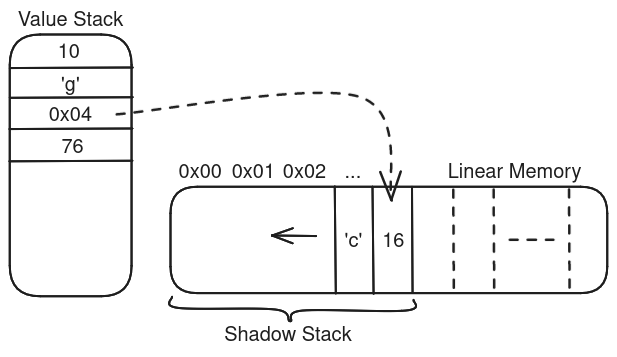
\includegraphics[width=0.5\linewidth]{value_and_shadow_stack.png}
  \caption{Value and Shadow Stack}
  \label{fig:value-shadow-stack}
\end{figure}

Those two stacks are present in the Wasm code but when it needs to be translated to the final bytecode the compiler tries to elide every access to the Value Stack allocating everything needed in the registers. Registers are limited though, so is impossible to use only them and the native stack of the embedder will be used if needed.

\

The main types of execution used in blockchains are: Ahead Of Time Complication (AOT), Just In Time Compilation (JIT), Single Pass Compilation and generally Interpretation


\begin{description}[font=$\bullet$ \scshape\bfseries]
  \item[AOT]
        is the standard compilation, all the code is compiled and then executed.
  \item[JIT]
        is a dynamic compilation type where the bytecode is compiled only when needed. The compiler needs to create first an intermediate representation, to be later able to compile the different parts only if the execution requires to. A really simple example to make is: we have a program with two entry point, function A and B. The JIT process will cover the understanding of the structure, recognize the two functions and compile only the needed one, either A or B.

        Lots of optimizations are already been done in the first phase of compilation, from the High-Level language to Wasm. In the second phase (runtime compilation) the main goal is to compile only the required parts to the machine-specific bytecode not caring too much about adding optimizations.
  \item[SPC]
        is a restriction of AOT Compilation, the complexity of the compilation must be O(n) so the Wasm bytecode will be scanned through only once. Like every other compilation methods here the objective is not to create efficient final code but to create the final bytecode as fast as possible.
  \item[Interpretation] % ???
        is the easiest way to execute Wasm, which becomes like any other interpreted language executed by a specialized Virtual Machine.

\end{description}

\subsubsection{Embedders}

There are multiple embedders able to execute Wasm using techniques not even explained before, we will focus on the embedders used in blockchains, they are Wasmtime, Wasmi and Wasmer.

Those three cover all the techniques just explained:

\begin{description}[font=$\bullet$ \scshape\bfseries]
  \item[Wasmtime]
        is a stand alone Wasm environment but it could be also used as library to create a Wasm environment in your bigger application. Wasmtime offers multiple features, it accepts Wasm in text or binary format and you're able to used JIT or AOT types of execution.
  \item[Wasmi]
        ~\cite{wasmi} is an efficient Wasm interpreter with low-overhead and support for embedded environment such as Wasm itself.

        There are multiple ways to interpret code, Wasmi makes a first Wasm bytecode pass to produce another stack-based bytecode, called WASMI IR (Intermediate Representation). Thereafter this representation is interpreted by a Virtual Machine, even with this transpilation it is only 5 times slower then the compilation to the native bytecode of the architecture.

        \item[Wasmer] has a lot of features, both AOT and JIT but in particular they implemented a single pass compiler for all the most important architectures.
\end{description}

\subsection{Security guarantee}

Wasm principle aim is to be extremely secure. The specifications describes a lot of ways to achieve that feature, but he security guarantee depends mostly on the execution. WebAssembly is designed to be translated into machine code running directly on the host’s hardware, so it can be sent to someone and be executed freely, (e.g., in browsers). We are running Wasm our machines every day, so security is a main concern.

Executing Wasm is potentially vulnerable to side channel attacks on the hardware level ~/cite{wasm-core-spec} and isolation is the only way to secure the execution.  The embedder translates one-by-one every instructions to native instructions on your computer, but nothing is dangerous if the code has no access to the environment where is executed.

The problem is that a completely isolation makes Wasm useless, so there must be a way to communicate with the environment or  have access to it, but those features are extremely limited and designed to be secure.

\subsubsection{Linear Memory}

From WebAssemply you have direct access to raw bytes, but where are  those bytes allocated? Wasm uses a MemoryObject provided by the embedder to describe the only accessible memory, besides the stack: the linear memory.~\cite{linear-memory}

Wasm does not have pointer types. Values in the linear memory are accessed as a vector, where the first index of the memory is 0.

Wasm, for security reasons that will be explained in the next chapters, works in a 32-bit address space. This makes usable only 4GiB of memory. Being the position of Linear Memory unknown to the Wasm blob every load or store to the memory is made passing through the embedder that will also do bounds checks to make sure the address is inside the Wasm Linear Memory.

\begin{figure}[h]
  \centering
  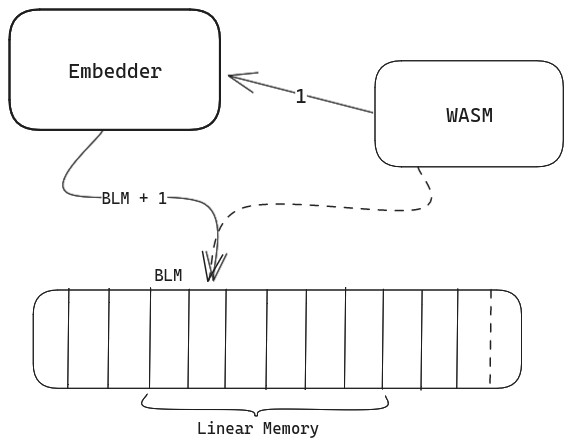
\includegraphics[width=0.5\linewidth]{linear_memory.png}
  \caption{BLM: Base Linear Memory Pointer}
  \label{fig:linear_memory}
\end{figure}

This level of control makes impossible to have memory leaks in the environment during the Wasm execution because there is a complete memory isolation. ~\cite{linear-memory}

\subsubsection{Communication in a sandboxed environment}

We just described how Wasm provides no ambient access to the computing environment in which the code is executed ~\cite{wasm-core-spec}, thanks to a mix of Wasm design choice and embedder implementation. But how  then the interaction with the environment works?

Every interaction can be done by a set of functions provided by the embedder and imported in the Wasm module~\cite{wasm-core-spec}. Those functions are called Host Functions and allow the Wasm code to access to resources, operating system calls or any other types of computation offered by the embedder. Generally the Exports provided by Wasm that are usable and callable from the embedder are called Runtime API.

\begin{figure}[h]
  \centering
  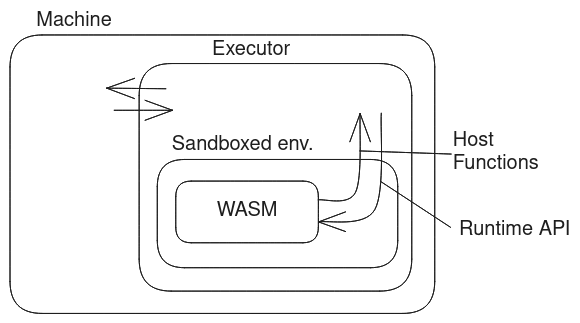
\includegraphics[width=0.5\linewidth]{env_communication.png}
  \caption{Environment communication}
  \label{fig:env-communication}
\end{figure}

\subsubsection{Wasmtime Security guarantee}

Wasmtime is widely used in different environments and as you will see in the next chapter one of those is the polkadot ecosystem.

Wasmtime main goals is to execute untrusted code in a safe manner.~\cite{wasmtime-book}

Some features that makes executing Wasm by Wasmtime secure are just inherited by the Wasm specifications. Some examples are: the callstack is inaccessible, pointers are compiled to offsets into linear memory, there's no undefined behavior and every interaction with the outside world is done through imported and exported functions.~\cite{wasmtime-book}

Wasmtime adds  a lot of mitigations to those features to limit risks:
\begin{itemize}
  \item Linear memories by default are preceded with a 2GB guard region
  \item Wasmtime will zero the memory used by a WebAssembly instance after it's finished.
  \item Wasmtime uses explicit checks to determine if a WebAssembly function should be considered to stack overflow
  \item The implementation language of Wasmtime, Rust, helps catch mistakes when writing Wasmtime itself at compile time
\end{itemize}

\end{document}


\clearpage{\pagestyle{plain}\cleardoublepage}
\chapter{Polkadot}
\label{chapter:polkadot}
\section{What's Polkadot?}

Polkadot is an heterogeneous multi-chain system~\cite{wood2016polkadot}. Its aim is to provide a scalable and interoperable framework for multiple chains with shared security.~\cite{burdges2020overview}

At the center of the entire system there is the `relay chain`, responsible for providing shared security to the other chains that are part of the system. Those chains are called `parachains`, they can be heterogeneous and independent between each others; the central point (relay chain) enables a trust-free inter-chain transactability and the pooled security.~\cite{burdges2020overview}

\begin{figure}[h]
  \centering
  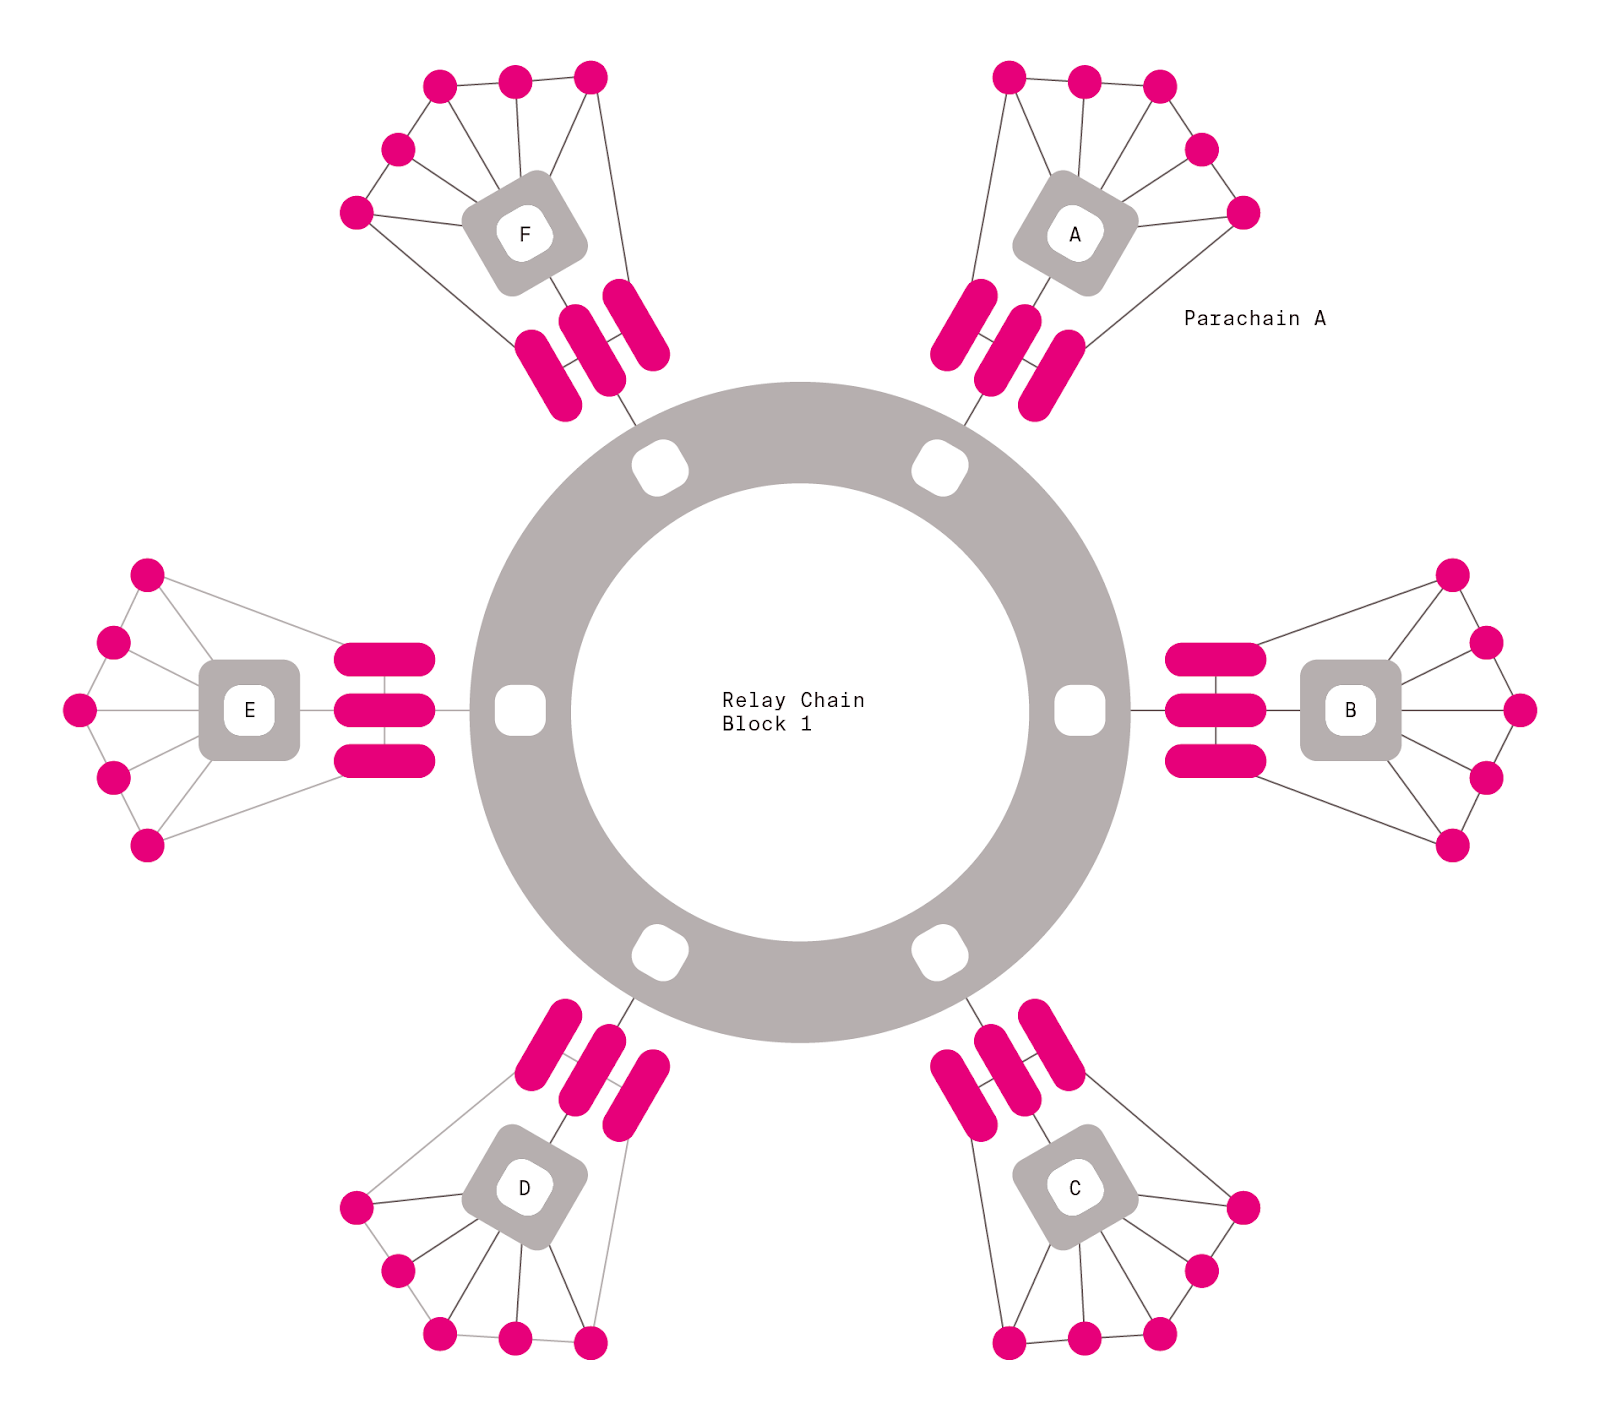
\includegraphics[width=0.7\linewidth]{polkadot_architecture.png}
  \caption{Polkadot's Architecture}
  \label{fig:polkadot_arch}
\end{figure}

Polkadot provides the bedrock relay chain upon which a large number of validatable, globally-coherent dynamic data-structures may be hosted side-by-side.~\cite{wood2016polkadot} What has just been described are the parachains that are not obligated to be blockchains, they  must just respect all the polkadot protocol.

In the Figure \ref{fig:polkadot_arch} you can see in the middle the relay chain that connects multiple parachains.

\section{Polkadot's protocol}

Briefly, the Polkadot system consists of a single open collaborative decentralised network (relay chain), that interacts with many other external chains (para chains)~\cite{burdges2020overview}. For the relay chain the internals of the parachians are not relevant, parachains need only to adhere to a specific interface. The relay chain then ensure that the parachain is trustable as a whole, not single nodes.

The ecosystem expects multiple actors to make the protocol work, the main are:
\begin{description}[font=$\bullet$ \scshape\bfseries]
  \item[Validator] Performs the bulk of the security work
  \item[Nonimator] Stakeholder who backs and selects validator candidates
  \item[Collator] Collects and submits parachain data to the relay chain
\end{description}

The protocol is composed by multiple phases and it defines the communication between parties. The main processes are:~\cite{burdges2020overview}

\begin{enumerate}
  \item The parachain's collators:
        \begin{itemize}
                \item Run full relay chain node to keep up the latest state
                \item Build new block on top of the latest state and submit blocks to the parachain's validator
        \end{itemize}
  \item The relay chain's validators:
    \begin{itemize}
      \item The ones associated to parachians produce the new relay chain block candidate
      \item Follow a sub-protocol to ensure data sharding, data are mainly parachain blocks and sharding is the process of making the validators collectively and robustly responsible for the availability of these blocks using erasure coding
      \item Submit votes to resolve forks and have a single head
      \item Manage messages between parachians
    \end{itemize}
\end{enumerate}

\subsection{State Transition Function}

The protocol's main goal is to verify what happened on parachains, described by the parachain logic. One of the few  thing trequired from a parachain is indeed that it implements a State Transition Function (STF). An STF describes the parachain logic and produces the transition between two states. Like any transaction-based transition system, Polkadot state changes via an executing ordered set of instructions, known as extrinsics.~\cite{burdges2020overview}

The STF is also present in every validator node because it describe the relay chain logic. Currently, all STFs are written in Wasm; for a parachain it would be theoretically possible to implement STFs with other PABs as well, but that would introduce additional complexities, as it will be illustrated in the following.

Every parachain or relay chain node can be divided into two parts: the STF (or Runtime) and the Client. The latter one implements everything else required to make the protocol work, from storage management to transaction gossiping.

Generally, the runtime is compiled into Wasm and stored as part of the state, this allows making fork-less upgrades because the code transition happens under consensus in the STF.

\section{Wasm in Polkadot}

Substrate is a framework to build blockchains, it is separate from Polkadot, and with it you're able to build so-called Solo Chains, a blockchain able to run on its own that does not care about the polkadot protocols.

Substrate is the main, and unique for now, framework used to build blockchains in the Polkadot ecosystem. Even the relay chain is built with substrate. Substrate abstracts all the complexity of writing client and runtime code. It provides almost everything at client level and leaves  the freedom of developing everithing else in the runtime, i.e. the specific state transition function of the specific blockchain under implementation.

Substrate compiles the runtime to Wasm and the client has an embedder, wasmtime, which is able to run the STF. As long as the chain is a Solo Chain, substrate manages everything, it compiles the runtime in wasm and implements all the custom logic to make the client and the runtime communicate through the embedder wasmtime.

The problems occurs when a blockchain wants to join the polkadot ecosystem, where there is pooled security, and the logic not only must be executed by the nodes that compose the parachain but also by the validators of the relay chain. This is made possible by following a protocol made by multiple phases that are built on top of two building blocks: the Parachain Validation Function (PVF) and the Proof of Validity (PoV).~\cite{parachain-protocol}

\subsection{PVF}

Using Substrate you end up with a Substrate-Runtime, which is  a wasm blob that implements the State Transition Function of the specific blockchain. To become a parachain you need to provide to the relay chain something that differs a bit from the Substrate-Runtime.

The protocol requires a Parachain Validation Function that is composed of the Substrate-Runtime and another function called 'validate\_block'. The reason why this function is required is related to a constraint of the relay chain: polkadot does not know anything about the previous state of the parachain.

Everything needed by the Runtime is not present in the validators node but is provided in the block proposed by the collators, that's called: PoV. The structure of the PoV will be explained later, but it is important to know now that every information needed in the execution of the PVF is indeed in the PoV.

The 'validate\_block' function is the glue between the parachain-runtime and the PoV. It accepts the PoV and reconstructs the previous state, applies all the extrinsics using the parachain-runtime and then checks that the new state is consistent with the one proposed by the collators.

Both relay chain and parachains implement the same HostFunctions for the runtime. This means that the STF of the parachain would access the storage through the same functions in the relay chain and in the parachain but what is known by the nodes is different.

As was just said the relay chain does not know the previous state of the parachain but the information resides in the PoV. The function 'validate\_block' overrides the host functions to let the STF access the reconstructed internal state, present in the PoV, instead of going into the relay chain client.

\begin{figure}[h]
  \centering
  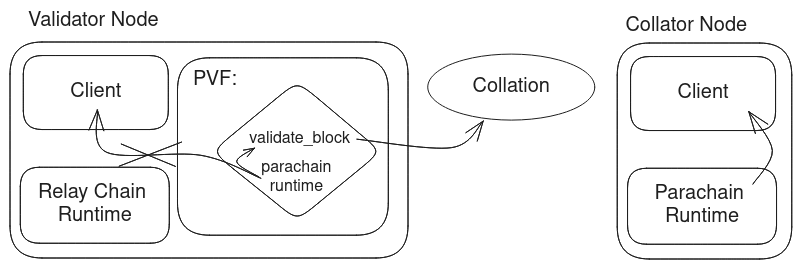
\includegraphics[width=0.8\linewidth]{validate_block_expl.png}
  \caption{PVF and Collation}
  \label{fig:pvf_pov}
\end{figure}

\'Collation\' is the term used to represent the outcome produced by the collators that will be used by validators, it is the same as PoV.

%maybe this is redundant

From the \ref{fig:pvf_pov} you can see how the parachain-runtime interacts in the same way with the embedder but it is different in the Collator or the Validator. In the first case the embedder is the client itself that knows the previous state, while in the Validator the embedder in the client is tweaked a bit so that the previous state is taken from the PoV and not from the Validator.

This encapsulation with a substitution of the host functions makes  validator able to execute different STFs without knowing anything about the parachain that is validating.

\subsection{PoV}

The Proof of Validity is made by all the things needed by Runtime Validation, it is mainly composed by:~\cite{cumulus-docs}

\begin{itemize}
  \item Header of the new block
  \item Transactions included in the block
  \item Witness Data
  \item Outgoing messages
\end{itemize}

The witness data is what makes it possible for the relay chain to execute the state transition validation without knowing the entire state of the parachain.

The state in polkadot is represented by a key-value database where each key is unique and there is no assumption on it. The database itself is arranged as a Merkle-Patricia Base 16 Trie that allows to describe the entire state in a single constant state proof. Each block stored in the relay chain contains the state proof of the previous block, and the witness data are then composed by:


% TODO: explain Merkle-Patricia Base 16 Trie ?
% maybe poit to the repo: https://github.com/paritytech/trie

\begin{itemize}
  \item Data used in the state transition by the collator
  \item Alongside their inclusion proof in the previous state
\end{itemize}

The Outgoing messages are everything that needs to be delivered to other parachains. The underneath protocol is XCMP following the XCM format which enables the parachain communication between parachains or with the relay chain.

\subsection{SmartContracts}

SmartContracts are arbitrary programs that can be uploaded on-chain and executed in the State Transition Function. Even though the STF is itself an arbitrary program that can be updated, SmartContracts add additional convenience by empowering final users to easily create and uploade custom logic on-chain. To implement SmartContracts different blockchains offer different solutions. Polkadot implements SmartContracts via a recursive embedder.


The Client is the embedder of the STF and the STF becomes itself the embedder of the SmartContracs. This is made possible thanks to Wasmi because it can be executed in wasm itself. There are different solutions to secure the execution of arbitrary, possibly malicious, code:

\begin{itemize}
  \item Gas / Fuel measuring
  \item Storage usage deposit
\end{itemize}

Where the first one aims at limiting the number of operations that can be executed in the STF, while  the second aims at limiting the amount of used storage.

\section{The crucial Role of Wasm in Polkadot}

Clearly, the distributed algorithms implemented in blockchains would be completely useless if nodes could not execute the code in a secure and deterministic manner.

The amount of tools and projects that are using Wasm makes it very suitable for polkadot, an environment with very constrained resources: there is limited space on every block, every state transition must be computed in a limited amount of time and multiple nodes must reach the same results. Wasm has already multiple tools like space and efficiency optimizer that make it even better for polkadot.

An important tools is Binaryen~\cite{binaryen} with the wasm-opt optimization phases, largely used in polkadot, that loads WebAssembly and runs Binaryen IR passes on it to make it more space and complexity efficient.

% \subsection{SPREE}


\clearpage{\pagestyle{plain}\cleardoublepage}
\chapter{Alternatives}
\label{chapter:alternatives}
Wasm is not the only PAB used in the blockchain space, other technologies use different solutions involving different protocols and algorithms. Examples are Ethereum with the custom PAB executed by the EVM (Ethereum Virtual Machine) or Solana that used eBPF to implement SmartConctracts, in the following section those solutions and others will be analyzed.
% TODO: Does Solana and eBPF should be cited here?

\section{EVM}

Ethereum Virtual Machine code ~\cite{buterin2014next} is one of the first PAB used in blockchain, it follows the principles used to describe a perfect PAB, it was created to be a perfect blockchain's bytecode and the Ethereum Virtual Machine is the glue that makes it executable on every machine.

The EVM is the main building block of the Ethereum technology, it executes stack based code and manage all the memory and access to the storage. EVM can be compared to a generic embedder for wasm with many features tied to the measurement of the computation on-chain, called gas.

\section{eBPF}

\subsection{What is eBPF}

Linux brought eBPF~\cite{ebpf} into the kernel, enabling sandboxed programs to run inside a privileged context (OS level). For lot of different reasons keeping the kernel upgraded was a difficult task and eBPF intend to solve this problem.

How can a new feature be developed once and be added to the Linux kernel? Keeping in mind that running arbitrary code developed by whoever in the kernel is absolutely not safe and the same code must be able to run on different architectures.

The operating system guarantee efficiency ans security through a JIT compiler and a verification engine for every eBPF program. To achieve that every kernel contains an eBPF VM able to checks the termination of the program and the security guarantees.

Main points of eBPF to make the verification process possible are:
\begin{enumerate}
  \item There are no functions in the code, there is only an unique blanket of code
  \item Limited control flow
  \item Loops need to be statically defined, they are unrolled at compile time
  \item The execution can't pass twice on the same code
\end{enumerate}

\subsection{Solana eBPF}

Not every program can compile to eBPF but a distributed systems need to execute arbitrary code and limitation as strict as normal eBPF are too much, Solana~\cite{yakovenko2018solana} then forked the eBPF backend of LLVM and removed lots of constraint, keeping the finality guarantee by the standard gas metering.~\cite{ebpf-contracts}

Solana also create a new virtual machine for eBPF, rbpf~\cite{rbpf}, able to: check, compile and execute the eBPF code on the blockchain.

eBPF is a perfect PAB for some use cases, as the linux kernel, but it does not seem to be a good fit for blockchains, examples are:
\begin{enumerate}
  \item limited control flow
  \item limited loops
  \item 64 bit usage implies lot of checks on the memory access
  \item 8 bytes instructions are too long
\end{enumerate}

\section{RISC-V}

RISC-V is a new instruction-set architecture (ISA)~\cite{risc-v-spec}, even if it is an actual bytecode for a specific hardware and seems to go against what has been described so far as PAB there are running experiments that makes this a valid option as PAB.

There are several reasons why RISC-V could be a good PAB even if it wasn't designed for:
\begin{description}[style=nextline]
  \item[Real ISA suitable for direct native hardware implementation]
        RISC-V is designed to be executed on real hardware, no assumption is made on the hardware itself, the only required thing is to respect all the constraint specified in the specifications. The ISA is developed following general machine patterns with something completely new but still very related to other machines making really easy the translation.
  \item[RISC]
        The name RISC stands for Reduce Instruction Set Computer, the specifications are then very small and simple making possible the creation of a base executor in really few lines of code.
  \item[Completely open ISA]
        RISC-V is an open standard, this makes possible to everyone to know the behavior and possibly create custom hardware to execute it.
  \item[ISA separated into a small base integer ISA]
        RISC-V is divided into smaller ISA, each one can work alone and can also be composed to achieve different functionalities. One of the most important division is the 32-bit and 64-bit address space division, it makes possible the creation of a sandboxed environment in an easy and effective way.
\end{description}

\subsection{RISC-V for SmartConctract}

One experiment~\cite{polkavm-forum} to port RISC-V in the Polkadot ecosystem as language for SmartConctract is polkavm-experiment~\cite{polkavm-experiment}.

The spec is so easy that creating an interpreter required only one day and the JIT only two days more. Those two executors were then tested against other PABs with different executors, everyone executed the same code: an NES emulator written in Rust and the interpretation was how close to 60 FPS the code can get.

The results are:
\begin{itemize}
    \item wasmi: 108ms/frame (~9.2 FPS)
    \item wasmer singlepass: 10.8ms/frame (~92 FPS)
    \item wasmer cranelift: 4.8ms/frame (~208 FPS)
    \item wasmtime: 5.3ms/frame (~188 FPS)
    \item solana\_rbpf (interpreted): 6930ms/frame (~0.14 FPS)
    \item solana\_rbpf (JIT): ~625ms/frame (~1.6 FPS)
    \item RISC-V interpreter: ~800ms/frame (1.25 FPS)
    \item RISC-V JIT: ~25ms/frame (~40 FPS)
\end{itemize}

As you can see the simplicity of RISC-V made possible the creation of a JIT compiler able to be faster than lot of competitive compiler already being used in different realities.

An important difference rather than eBPF is dedicated instructions for syscall (used as Host Function in the SmartContract) and the support in rustc and LLVM. One of the main constraints is the number of registers used in RISC-V, 32 registers while most architectures use 16, the compiler or interpreter then must properly manage those extra registers.


\clearpage{\pagestyle{plain}\cleardoublepage}
\chapter{Conclusions}
\label{chapter:conclusions}
\section{BOH}
\subsection{still boh}


\clearpage{\pagestyle{plain}\cleardoublepage}
\bibliographystyle{plain}
\bibliography{refs}

\end{document}
